\chapter{Intensity Extraction \& Fourier Maps}\label{Chap:intextraction}

In this chapter I will talk about how reflection intensities are estimated, including two intensity fitting methods, Pawley and Le Bail fits and then finally things that you can do in GSAS-II using the extracted intensities. 

\section{Rietveld's Intensity Extraction Method}

One long-standing problem back in the 1960's, when Hugo was busy developing Rietveld refinement, was how to come up with an estimate for the ``observed'' structure factors, $|F_{obs, hkl}|$, from a powder diffraction pattern. These estimated observed structure factors would allow one of the more common crystallographic computations, Fourier maps, for structure completion as will be discussed in section \ref{ref:Fourier}. While I don't find them usually very useful from powder diffraction, with ``observed'' structure factors one can compute Patterson maps which might allow structure solution for ``heavy atom'' powder diffraction patterns. 

Estimating the area under a peak was not a problem, but how to apportion out that intensity when a peak was composed of overlapped reflections posed a challenge. This could be done by use of deconvolution for peaks that were separated by a reasonable fraction of the FWHM, but even so deconvolution, but that was slow back in those days. However, when reflections are exactly or very nearly overlapped, the peak intensity can be divided amongst the reflections in any manner. 

As part of his original software, Hugo Rietveld came up with a method for estimating  ``observed'' structure factors, $|F_{obs, hkl}|$ which has also become universal in the field. I have referred to this as ``Hugo Rietveld's other breakthrough'' and it is a quite nice technique. In order to compute the powder diffraction pattern, Hugo's software first had to compute structure factors from the model, $F_{calc, hkl}$, these then multiplied by the profile function, the multiplicity and finally other scaling constants, such as the Lorentz-Polarization correction, the scale factor and the phase fraction and that product determined how much intensity to add to a given point in the calculated powder diffraction profile. This was done for every reflection and every data point in the pattern. In the end, that meant for every point in the computed diffraction pattern it could be tracked how much of that intensity came from each reflection. The beauty of Hugo's intensity extraction algorithm was that he just turned that computation around. For every point in the \textit{observed} powder diffraction he used the same factor applied to the $F_{calc, hkl}$ and used that to divide each data point's actual intensity and added that to the variable that would in the end contain the estimate for $|F_{obs, hkl}|$. For convenience, the peak shape function is normalized to unit area. 

This may not do a perfect job with two overlapping peaks, where $|F_{obs, hkl}|$ and $|F_{calc, hkl}|$ are closely matched for one reflection and not the other, but will put most of the extra intensity into the right reflection. With completely overlapped peaks, it will divvy up the extra intensity weighted by the multiplicity. Perhaps not correct, but there are no better \textit{ad hoc} choices. I don't believe anyone has improved over this algorithm in newer implementations of Rietveld fitting. As it turns out, for many years when I presented this intensity extraction method in my introduction to Rietveld analysis, I did this with a slide titled, ``Hugo Rietveld's other breakthrough.'' I wonder if that slide prompted the e-mail that I very much prize that is reproduced in Fig. \ref{fig:Hugo}.  Note that 20 years later, none of the links in the e-mail still work, but a version of my slides are still online\footnote{see https://www.aps.anl.gov/files/APS-Uploads/Education/Powder-Diffraction/RietveldIntro.pdf}.

\begin{figure}
    \centering
    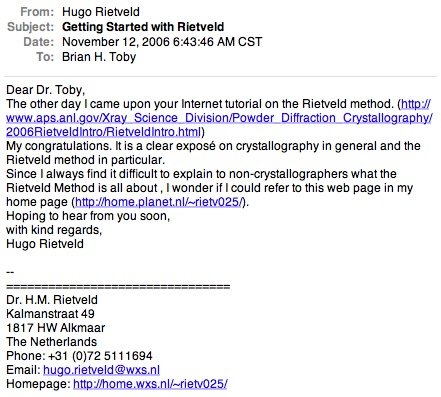
\includegraphics[width=0.75\linewidth]{figures/Hugo.jpg}
    \caption{Brian showing off: Fan mail from Hugo! Note that the links in this e-mail no longer work.}
    \label{fig:Hugo}
\end{figure}
\section{Fourier Maps}\label{ref:Fourier}

As was explored in section \ref{ref:rho}, if we know the structure factors, including their phases, we can use the Fourier inversion of the structure factor equation,
$$\rho(x,y,z) = \frac{1}{V} \sum_{hkl}  F_{hkl} \exp⁡[-2πi(hx + ky + lz)] $$
and obtain the scattering strength at any site in the unit cell. When this is computed for a three-dimensional grid of points across the unit cell (or better, just the unique portion of the unit cell) we get what is known as a Fourier map. The locations that have the most density are where there must be scattering matter (electrons or nuclei) in the crystal. If we use the $F_{calc, hkl}$ values in this equation, we get back the rather uninteresting result of a map that shows the positions of the atoms that were used to compute the $F_{calc, hkl}$ values. This is known as a Fcalc map.

We cannot directly use the $|F_{obs, hkl}|$ values that we discussed tabulating in the previous section because those values are unphased magnitudes, but we can use the quantity  $\frac{F_{calc, hkl}}{|F_{calc, hkl}|}|F_{obs, hkl}|$ to compute the map. This is known as a Fobs map. What this does is use the phases we computed from our structure, but the approximate observed intensities. Although this map is only approximate, for several reasons, including that the $|F_{obs, hkl}|$ values are only approximately correct and that the phases we compute for $F_{calc, hkl}$ will not always be the correct phases for $|F_{obs, hkl}|$ in addition to the truncation errors previously mentioned. Nevertheless, map would be expected to show any atoms that are missing from our model, as well as the atoms included in the model. 
The most valuable map that is commonly computed is obtained from $\frac{F_{calc, hkl}}{|F_{calc, hkl}|}(|F_{obs, hkl}| - |F_{calc, hkl}|)$ and is known as a $\Delta$F map, delt-F map or an obs-calc map. This requires a bit of thought to understand, but it gives us positive peaks any place in the cell where there are atoms present that are not included in our model. Should there be scattering in our model where there is less or no actual scattering present in the material, then the $\Delta$F map will have negative peaks. Thus, a negative peak can be diagnostic for the misassignment of an atom type or the presence of vacancies. When an atom is slightly shifted from its actual position, a negative peak will be seen next to the actual atom location. 

Note that for neutron scattering, a small number of isotopes scatters with a negative scattering length. For those atoms the sign of the Fourier peak is inverted. In a $\Delta$F map, a negative peak means that more of that atom is needed and a positive peak indicates too much density. It is possible with site sharing for the atomic scattering to sum to zero and then nothing will be seen on a Fourier map for that site.

There is are other types of maps that GSAS-II can produce. If the quantity $\frac{F_{calc, hkl}}{|F_{calc, hkl}|}(2|F_{obs, hkl}| - |F_{calc, hkl}|)$  is used, known as a ``2Fo-Fc'' map, then one sees the missing atoms superimposed, but at double intensity, on the map with the atoms from the model. This is a preferred mode for Fourier map analysis in macromolecular crystallography, but I have not found it particularly useful for my powder diffraction analysis work. In macromolecular crystallograph, one sometimes removes an amino acid from a model to see where the is then found in the Fourier map, to better determine the position and orientation. This is called an ``omit map.''  This can be done in GSAS-II, but will not be discussed here. 

Finally, GSAS-II can compute a Patterson map, where the quantity  $|F_{obs, hkl}|^2$ is used for  $F_{hkl}$ in the summation. This gives a map where peaks correspond to vectors between pairs of atoms and the strength of the map peaks goes as the product between the scattering power from each type of atom in the pair. While not used very much at present, Patterson maps were commonly used for solving structures of ``heavy atom'' materials from single-crystal data, but as direct methods have improved for these types of materials, Patterson maps do not see much use. It is possible that it might be a useful tool for certain powder diffraction problems, but the one time I did try to use it for that, it did not give me what I needed. Analysis of a Patterson map requires several ``tricks'' that I will not try to resurrect my memories from when I did solve structures with this in the 1970's, but one can consult the older scientific literature, which is rich with Patterson technique information. 

In my experience, powder diffraction Fourier maps are not as accurate as those from single-crystal diffraction. I assume this is due to peak overlap. What I find is that only the first few peaks in a map are real and the rest tend to represent artifacts. I will examine the most intensely positive and negative regions of a $\Delta$F map, assigning atoms where possible, and then perform a refinement. I will then recompute the Fourier map and again look at the most and least intense regions, until I have nothing more to change. 

Computing a Fourier map in GSAS-II is quite easy. 
\begin{itemize}
    \item The first step is that one must compute the powder diffraction pattern using the Compute/Refine menu command. It does not matter if any cycles of least-squares are performed, but the use of Compute populates the histogram reflection lists. 
    \item Set the Fourier map settings. These are on a phase's General tab. 
    \begin{itemize}
        \item The first thing to select is the map type. My recommendation when looking for problem aspects of a refinement is to use a delt-F ($\Delta$F) map. 
        \item Then select the reflections to use in the map computation by clicking on the ``Select reflection sets'' button. You can then select one or more histograms to use for structure factors. You will typically use only one histogram, but if your data were collected in segments, you can select more than one histogram. If a reflection is found in more than one selected histogram, I believe the last value that is found is the one that is used, but I am not certain on this. 
        \item The ``Map grid step'' is the spacing for the grid for the map: the default value of 0.25 $\mathring{\text{A}}$ is usually a good choice as it will place at least few points in the vicinity of every atom. 
        \item The peak cutoff value will be used later when we search the map for Fourier peaks and will be discussed later
    \end{itemize}
    \item     Use the Compute/``Fourier map'' menu command and the requested Fourier map is then computed. This goes very quickly, If you look at the console you will see a message with the maximum and minimum $\rho$ values in the map. 
\subsection{Viewing a Fourier map}
\end{itemize}

The Fourier map can be viewed directly, superimposed on the desired representation of the structure, by selecting the ``Draw Options'' or ``Draw Atoms''. Before viewing the Fourier map, you should prepare the structure as you wish to view it. For details on that, please see  Chapter \ref{Chap:structureplotting}. 

Note that the ``view point'' is important for selecting what section of the map is displayed. The view point is placed in the center of the graphics window. If the ``Show view point'' option is selected in the ``Draw Options'' tab, it is drawn with 1 $\mathring{\text{A}}$ lines along the \textit{a}, \textit{b} and c, directions, with the lines colored red, green and blue, respectively. The location of the view point can be set in a number of ways:
\begin{itemize}
    \item Values can be typed into the  ``View Point'' box on the ``Draw Options'' tab. Press enter or click elsewhere for the values to be used.
    \item Drag the right mouse button, this will displace the view point in the screen's x-y plane. Alternate use of the left mouse (which rotates the structure around the screen's x \& y axes) and the right mouse to position the view point in three dimensions. 
    \item Pressing the ``c'' keyboard key will reset the view point to its default, which is ($\frac12,\frac12,\frac12$).
    \item With the ``Draw Atoms'' tab selected, you can select one or more atoms from the table and then use the ``Edit Figure''/``View Point'' menu command. The view point will be placed on the selected atom. Or, if more than one atom has been selected, at the point midway between the selected atoms. If no atoms have been selected before the ``Edit Figure''/``View Point'' menu command is invoked, a dialog window is opened where atom(s) can be selected. 
    \item It is also possible to move the view point to Fourier map peaks, as will be described later. 
\end{itemize}

There are two modes that can be used to view the map, as discussed below: 

\subsubsection{Viewing the map as a 3-D object}
GSAS-II can display the Fourier map in three dimensions for a spherical region surrounding the view point. Positive regions are shown as green dots and negative regions are shown as orange dots. The higher the level, the more dense the dots. See Fig. \ref{fig:Map3D} for an example. To display the map in this fashion, on the  ``Draw Options'' tab select the ``Show 3D density map''  option. There are then two controls that dictate how the map shown. There is a ``Fraction of rho max'' slider that can have values from 1.0 to 0.01. The lower the value, the more of the map that will be shown. Regions where $|\rho|$ is below this threshold are not displayed. One can also select the radius of the sphere using the ``Radius of displayed map'' slider/input box. 
\begin{figure}
    \centering
    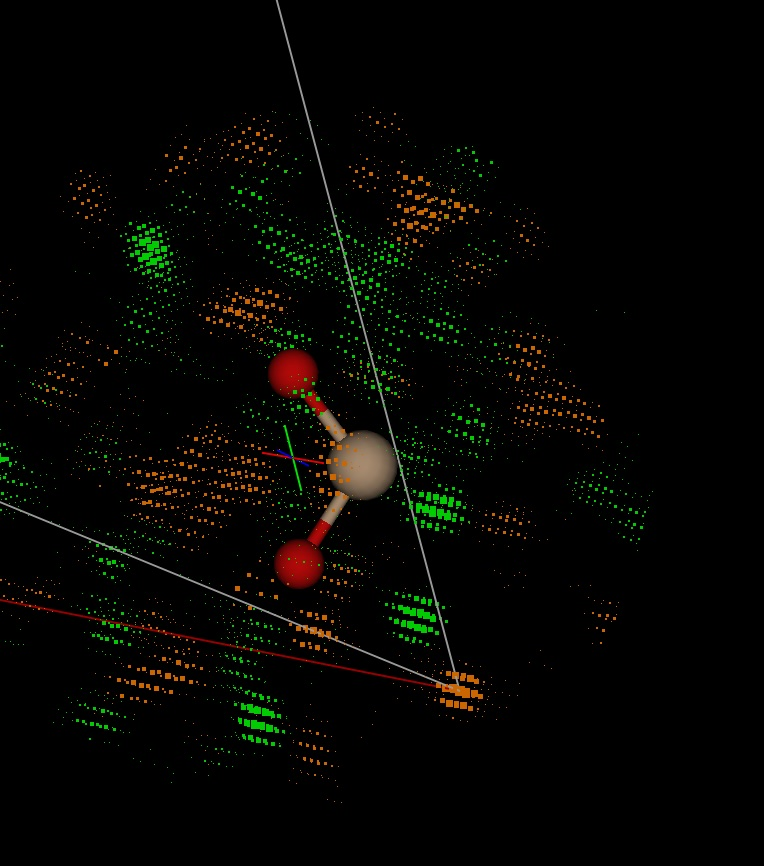
\includegraphics[width=0.6\linewidth]{figures/Fourier3D.jpg}
    \caption{A view of a Fourier map as a 3-D object. The map is being drawn as a 5 $\mathring{\text{A}}$ sphere around a water molecule.}
    \label{fig:Map3D}
\end{figure}
\subsubsection{Viewing the map as a 2-D slice}
The map can also be displayed as a 2-D slice. The slice will always viewed in the plane of the screen and will always be centered on the view point, so rotating the structure with the left mouse button changes the orientation of the plane. . See Fig. \ref{fig:Map2D} for an example. The plane can be enabled by selecting the display option for the ``Show map slice as...'' on the  ``Draw Atoms'' tab between lines, colors and lines+colors. Pressing the ``k'' keyboard key also toggles between these modes. One can also select the slice size and the contouring levels. 
\begin{figure}
    \centering
    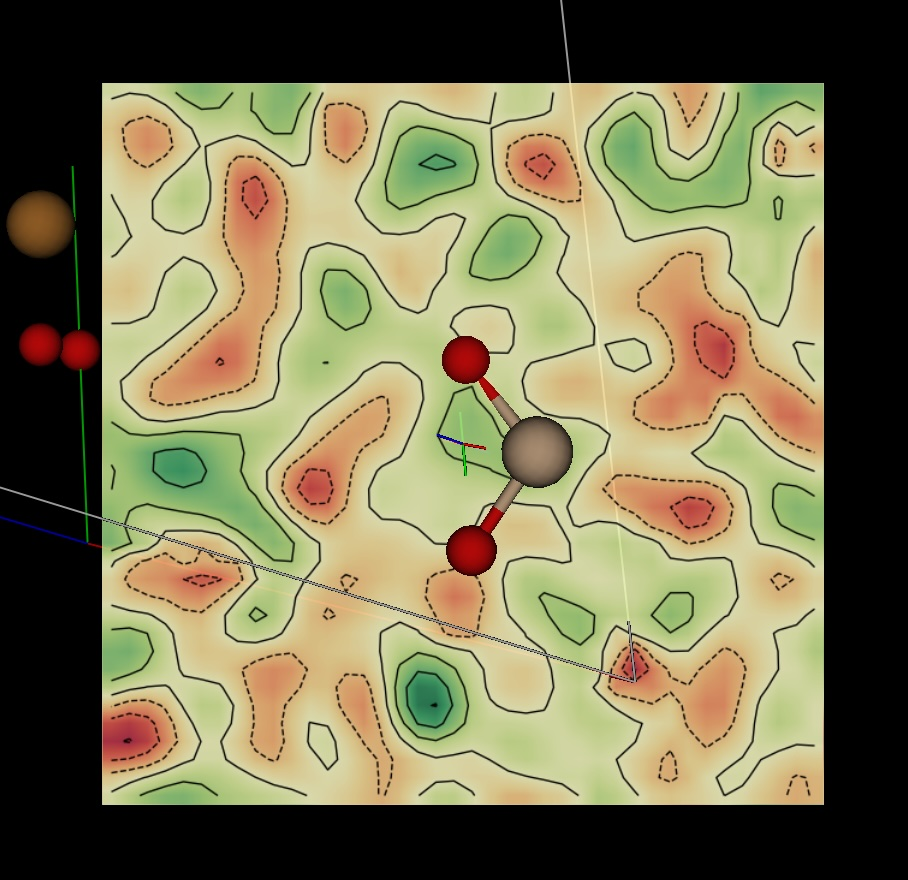
\includegraphics[width=0.6\linewidth]{figures/Fourier2D.jpg}
    \caption{A view of a Fourier map as a 2-D map slice. The map is being drawn as a $5 \mathring{\text{A}} \times 5 \mathring{\text{A}} $ contour plane around a water molecule.}
    \label{fig:Map2D}
\end{figure}

\subsection{Working with map peaks}

I find that when I am using Fourier maps, my primary goal is to identify where the most and least intense Fourier densities are located in the structure. To do this it is useful to identify the regions with the most positive and  negative Fourier densities. GSAS-II can search the map and assemble a list of Fourier peak locations as well as the density at that location. To do this, on the ``General'' tab use the Compute/``Search map'' menu command. The number of peaks located will be determined by the ``Peak cutoff \%'' option. If rho-max is 0.8 and this threshold is set to 50\%, then only peaks with $\rho > 0.4$ or $\rho < -0.4$ will be located. The peaks will be listed on the ``Map peaks'' tab and will be displayed superimposed on the structure as small cross marks. Lines are drawn between peaks, which may help one recognize molecular fragments, but mostly that is of use for charge flipping structure solution, and not so much for Fourier maps. 

When the peak list is viewed in the ``Map peaks'' tab, the structure/map display can be updated as peaks are selected, according to options on the  ``Draw Options'' tab:
\begin{itemize}
    \item If ``On map peak selection... move view point'' is selected, then as a map peak is selected, the view point is moved to the map peak, centering the plot around that point.
    \item The value for ``Show map points'' will generate other Fourier map peaks applying symmetry if needed, for any map peaks that occur within the specified distance, if non-zero.  
    \item The value for ``Show atoms within'' will generate atom positions, applying symmetry if needed, for any atoms that are within the specified distance, if non-zero.
    \item   The value for ``Label distance to atom within'' causes the distances to atoms and Fourier map peaks to be labeled when less than this amount. 
\end{itemize}
Peaks can be selected by clicking on them in the ``Map peaks'' data tab. Pressing the ``n'' and ``p'' keyboard keys in the graphics window selects the next or previous Fourier peak. 

Note that if the view point is moved around the cell, it is possible to locate atoms and Fourier peaks, as well as label distances, with a set of options that work similarly to those immediately above. 

\subsection{Are map peaks real?}
My experience with Fourier peaks from powder diffraction is that they do not always correspond to actual atomic positions. Peaks that are close to an atom that is already in the structure may send a hint that there is something lacking in the fit for that atom, but could also be an artifact. The hint could be nothing significant, but could be an indication of some disorder or perhaps that the atom has significantly anisotropic thermal motion. There may not be anything that one can change. When I encounter a peak that is sufficiently remote from other atoms in the structure that it could be bonded to atoms in the structure, or if even further than that I will wonder if there is an additional atomic fragment or a solvent, etc. Note that other than intentionally porous materials, it is fairly rare for structures to have open voids large enough to accommodate atoms or molecular fragments. I will often test if placing an atom at that location actually improves the fit. This is fairly easy: Place an atom at that site and vary the occupancy, but not Uiso or coordinates. If the model is not improved by scattering from the site, the occupancy will refine to a value close to zero. If it refines to a small positive number that is well beyond several times the uncertainty for the occupancy value (which can be checked in the .lst file) I will withhold judgment on if I believe there really is an atom at that location until later. It is worth noting that an easy way to create an atom at a map peak location is to use the option to move the view point to a selected Fourier map peak. Then select the Atoms tab and use the ``Edit Atoms''/``Append view point'' menu command. That places a H atom at the view point location. One can then click on the H in the Type column for the new atom and a periodic table will be presented where the atom type can be changed. 


\section{Pawley Fitting}\label{ref:Pawley}\index{Pawley fitting}
There are effectively two approaches to fitting x-ray diffraction patterns. In Rietveld fitting, peak positions are determined from a phase's lattice parameters and intensities are determined from the crystallographic structure. In the second approach, individual peak fitting, which is also called sometimes called pattern deconvolution, both the peak positions and the peak intensity are treated as independent varied parameters. Peak profiles may or may not be treated as individual variables. GSAS-II implements both methods, where peak fitting is discussed in Chapter \ref{Chap:peakfitting}. In the late 1970's Stuart Pawley\index{Pawley, S.} developed a program he called ALLHKL that blended the two approaches. Peak positions were determined from lattice parameters, but peak intensities were fit directly as least-squares variable parameters. A bit of finesse was needed to decide when two reflections were too closely overlapped to deal with as individual reflections, but use of lattice parameters to determine peak positions is greatly advantageous when one has two closely-spaced peaks. Without that constraint, the peak tends to be fit as a single peak somewhere between the two actual positions. Note that in a Pawley fit, all of the usual parameters that determine background, peak positions and peak shapes can be refined in conjunction with the parameters, but care should be taken to only refine those terms after fairly good fits are obtained for reflection intensities. Parameters that determine peak intensities, such as atomic positions, texture or scale factors cannot be refined in a Pawley fit, of course.

The result of a Pawley fit provides an ideal fit to the crystallographic fit to a powder diffraction pattern, in that all reflection intensities are optimized to provide the best fit possible, which would match that of an ideal crystallographic model. The use of a Pawley fit provides a good starting point for fitting the non-crystallographic parameters, as has been discussed in Chapter \ref{Chap:profile}. Likewise, as has been discussed in section \ref{ref:beststruturefit}, at the final stages of a refinement project, a Pawley fit provides a measure for what R-factor or reduced $\chi^2$ value would be obtained in an ideal crystallographic fit, taking into imperfections in peak shapes, background fitting, etc. A Pawley fit can also be used to subtract out peaks from an impurity phase that has a known unit cell, but not a known structure, or for a phase that will not be fit well due to texture. Aluminum sample cans in neutron diffraction are an example of the latter case. 

It should be noted that a Pawley reflection intensities are tied to the phase definition, so that if a phase is associated with more than one histogram, the same set of reflection intensities is used for all histograms. If you have very different types of datasets, this is probably not what you want do.  

Setting up a Pawley fit in GSAS-II requires a few steps. First, you should look at the histogram(s) used in the phase to look at the data range that is needed, in my dreaded d-space units. You want to find the maximum d-space that includes the lowest Q peak across all histograms. Note that at the status line at the bottom of the GSAS-II graphics window, the $2\theta$/TOF position of the cursor is shown, along with the corresponding Q value and d-space values. Also do this for the high Q region, but be careful to stay very close to the minimum d-space. You will use these values to generate a list of reflections and you do not want to generate any reflections that are outside the region(s) where you are going to fit. 

For the next step, use the ``Select tab''/``Pawley Reflections'' (or use the arrows on the tab bar to scroll to this tab). The data window will give you a hint for the next step, which is to use the Operations/``Pawley setup'' menu command. The modal window shown in Fig. \ref{fig:pawley1} will be opened. Select the ``Do Pawley refinement'' flag to be on, if that is not already set, and type in the range of as d-space values that you previously determined. 
\begin{figure}
    \centering
    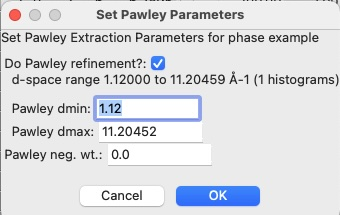
\includegraphics[width=0.4\linewidth]{figures/pawley1.jpg}
    \caption{Window created by ``Pawley setup'' menu command.}
    \label{fig:pawley1}
\end{figure}
After closing the previous window by pressing OK, a window will be created, shown as Fig. \ref{fig:pawley2},  asking if you want to create a table of reflections to be used in Pawley fitting. Press the ``Yes'' button. (This step can be done manually using the Operations/``Pawley create'' menu command.) This will also also the intensities of in this table to good starting values. (That step can be repeated at any point using the  Operations/``Pawley estimate'' menu command.)  The window will now be filled with a list of reflections, as seen in Fig. \ref{fig:pawley3}.  Note that in this window, double-clicking on the ``refine'' column label brings up a menu where the refine flag for all reflections can be set. 
\begin{figure}
    \centering
    
\includegraphics[width=0.25\linewidth]{figures/pawley2.jpg}
    \caption{Reminder window created after using ``Pawley create''.}
    \label{fig:pawley2}
\end{figure}
\begin{figure}
    \centering
    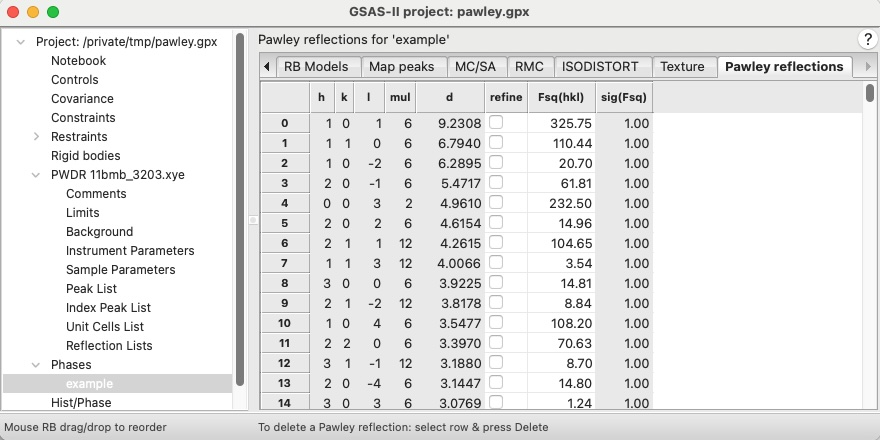
\includegraphics[width=1\linewidth]{figures/pawley3.jpg}
    \caption{Table of Pawley reflections created using the ``Pawley setup'' menu command.}
    \label{fig:pawley3}
\end{figure}
At this point, a refinement can be performed where the reflection intensities can be refined. Be sure to turn of refinement of all structural parameters, as well as any other parameters that change reflection intensities. 

\section{Le Bail Fitting}\label{ref:LeBail}\index{Le Bail fitting}
Armel Le Bail\index{Le Bail, A.} came up with another implementation for pattern-fitting in the late 1980's that avoids use of least-squares refinement for reflection intensities and cleverly takes advantage of Hugo Rietveld's intensity extraction method. He wanted $|F_{obs, hkl}|$ values for materials where he wanted to determine the structure, and thus had no idea for information to provide approximate $F_{calc, hkl}$ values, but did have a known unit cell. He ran a Rietveld fit where instead of computing all the $F_{calc, hkl}$ from the structure, he overrode the computed values and set them all to a constant. After this was done, computing the powder pattern was done and as expected the match to the pattern was terrible. Hugo's intensity extraction method could still be used to come up with estimates for the $|F_{obs, hkl}|$ values. They would be imperfect, but certainly far better than the constant values he started with for $F_{calc, hkl}$. He then replaced the previously constant $|F_{calc, hkl}|$ values with the just-extracted $|F_{obs, hkl}|$ values and then recomputed the diffraction pattern. The match between the observed and computed patterns would now be much closer. Likewise, repeating the intensity extraction gave even better values than those from before. This process would be cycled a few times resulting in a pattern is that is well-fit and a good set of $|F_{obs, hkl}|$ values is obtained, though the intensities for overlapping peaks will be apportioned a bit differently than in the Pawley method. Once the intensities have been fairly-well fit, it is also possible to refine background, peak positions and peak shape parameters rather than simply recomputing the pattern. 

It should be understood what this Le Bail process is doing. The Le Bail extraction process is effectively a steepest descent fitting method for reflection intensities while if any parameters are being fit, that is being done via Levenberg-Marquardt damped Gauss-Newton fitting, but that fitting process is completely disconnected from the intensity fitting process. This type of fitting is not very stable if the parameters are undergoing large changes, which is why it is wise to approach Le Bail fitting with a ``soft touch.''

Bob Von Dreele came up with an alternate approach to Le Bail fitting, where instead of setting all $F_{calc, hkl}$ values to a constant, they remain at whatever values they have been computed at, based on the structural information in the model. This is useful when a partial structure is known. In this case, the $F_{calc, hkl}$ values from the partial structure are likely to be better starting guesses than setting all values to a constant. 

You should understand that Le Bail intensities are optimized in GSAS-II when the powder profile is computed, even if no least-squares optimization cycles are performed. Setting the number of least-squares cycles (in the Controls data tree item) to 0 and then using the Calculate/Refine menu command will optimize the Le Bail intensities.  Doing this twice is usually enough to bring the intensities pretty close to optimum values. At this point the number of cycles can be set to a non-zero value, but it is wise to add parameters to the fit slowly due to the potential instability of the fitting process. 

Note that unlike the Pawley fitting, which is a phase property, Le Bail fitting is a HAP setting, so that Le Bail fitting can be done for only for selected histograms associated with a phase. Also, each histogram for each phase has an independent reflection table, so Le Bail intensities are not shared across histograms. 

To perform a Le Bail fit, go to the Phase’s Data tab (or in “SeparateHistPhaseTreeItem” mode, in the Hist/Phase data tree item) and press the ``Start Le Bail extraction'' button, just under the plot selection options. When the Calculate/Refine menu command is first used after Le Bail is selected, the window seen in Fig. \ref{fig:LeBail1} is displayed, where you are offered a choice for how the Le Bail extraction is initialized. When ``Yes'' is selected here, all reflection intensities are initialized (as in the original Le Bail method), but if ``No'' is used, the Von Dreele approach is used, where the previous $F_{calc, hkl}$ are used as starting values. A Le Bail-only fit is then performed, where the powder diffraction pattern is computed, but no parameters are optimized. A window will be opened with results from this fit and you will be asked if the fit should continue with refinement of parameters. Note that these two steps are only performed when Le Bail mode is initially turned on. In subsequent refinement steps, the reflection intensities are not reset and no ``Le Bail-only fit'' is performed, but should the latter be wanted, this can be done by setting the number of least-squares cycles to 0. 

\begin{figure}
    \centering
    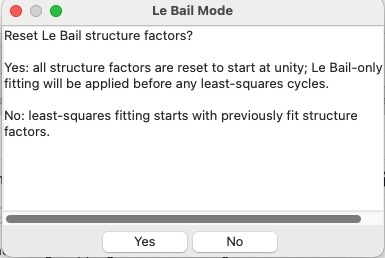
\includegraphics[width=0.35\linewidth]{figures/LeBailInit.jpg}
    \caption{Window to select a choice for initializing the $F_{calc, hkl}$ values for a Le Bail fit.  ``Yes'' selects the original Le Bail method where all values are set to 1 and ``No'' uses the Von Dreele approach, where the stucture input is used.}
    \label{fig:LeBail1}
\end{figure}
